\documentclass[border=6pt]{standalone}
\usepackage{amsmath}
\usepackage{amssymb}
\usepackage{tikz}
\usepackage{xcolor}
\usetikzlibrary{arrows.meta,calc,positioning,shapes.geometric}
\begin{document}
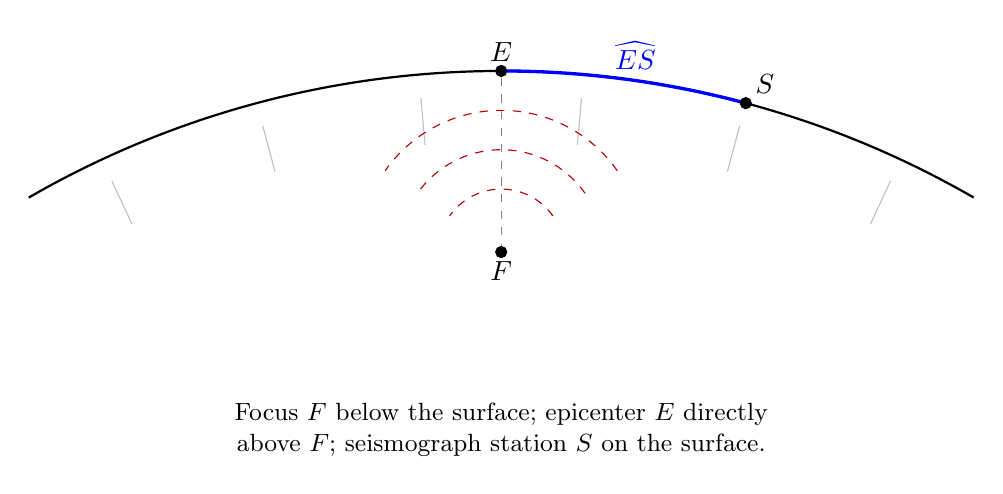
\begin{tikzpicture}[font=\sffamily]
  \coordinate (C) at (0,-12);
  \def\R{12}

  % ground / surface arc (plain)
  \draw[thick] ($(C)+(60:\R)$) arc (60:120:\R);
  % subtle cutaway hatching below the surface
  \foreach \a in {65,75,85,95,105,115}{
    \draw[gray!50] ($(C)+(\a:\R-0.3)$) -- ($(C)+(\a:\R-0.9)$);
  }

  % focus F (below the surface), epicenter E (on surface, directly above F),
  % station S (elsewhere on the surface)
  \coordinate (F) at (0,-2.3);
  \coordinate (E) at ($(C)+(90:\R)$);
  \coordinate (S) at ($(C)+(75:\R)$);

  % highlighted arc ES -- the surface segment between E and S
  \draw[very thick, blue] ($(C)+(75:\R)$) arc (75:90:\R);

  % dashed line: focus straight up to epicenter
  \draw[dashed, gray] (F) -- (E);

  % radiating dashed wave-arcs from the focus
  \foreach \r in {0.8,1.3,1.8}{
    \draw[dashed, red!70!black] (F) ++(35:\r) arc (35:145:\r);
  }

  % points and labels
  \filldraw[black] (F) circle (2pt) node[below] {$F$};
  \filldraw[black] (E) circle (2pt) node[above] {$E$};
  \filldraw[black] (S) circle (2pt) node[above right] {$S$};
  \node[blue] at ($(E)!0.5!(S)+(0.15,0.4)$) {$\widehat{ES}$};

  \node[align=center, text width=9cm, font=\small, below=1.8cm of F]
    {Focus $F$ below the surface; epicenter $E$ directly above $F$;
     seismograph station $S$ on the surface.};
\end{tikzpicture}
\end{document}
